\documentclass{beamer}
\usepackage[utf8]{inputenc}
\usepackage[T1]{fontenc}
\usepackage[brazilian]{babel}
\usepackage{amssymb}
\usepackage{amsmath}
\usepackage{multirow}
\usepackage{graphicx}
\usepackage{caption}

\graphicspath{{./imgs/}}

\setbeamertemplate{caption}[numbered]
\setbeamercovered{transparent}

\usetheme{Warsaw}
\usecolortheme{default}

\title{Movimento e dinâmica} 
\author[Paulo Pinheiro]
{Dr. Paulo Pinheiro\inst{1}}
\institute[UNIFAP]
{
    \inst{1}
    Centro Universitário Paraíso do Ceará\\
    UNIFAP
}
%
\date{Última atualização:\\ \today}
\logo{\large \LaTeX{}}
\logo{
\includegraphics[height=0.8cm]{UNIFAP.png}}
%
\begin{document}
% Title page frame
\begin{frame}
    \titlepage 
\end{frame}
%
% Remove logo from the next slides
\logo{}
% Outline frame
\begin{frame}{Outline}
    \tableofcontents
\end{frame}
%--------------------  FRAMES  ------------------------
%%
% Lists frame
%%
\section{Introdução à disciplina}
%
\subsection{Ementa da disciplina}
%
\begin{frame}
    \begin{block}{Ementa}
        Caracterização das grandezas físicas.\\
        Estudo das medidas e medições lineares.\\ 
        Análise gráfica de fenômenos físicos. \\
        Estudo de vetores. \\
        Estudo dos movimentos em uma, duas e três dimensões. \\
        Introdução à dinâmica e estática de partículas. \\
        Caracterização das relações entre trabalho e energia mecânica. \\
        Elaboração de experimentos de sistemas físicos reais.
    \end{block}
\end{frame}
%
\subsection{Instrumentos e critérios de avaliação}
%
\begin{frame}{Notas}
    
\end{frame}
%
\subsection{Conteúdo programático}
%
\begin{frame}{Formação inicial 1}
    \textbf{Conceitos iniciais}
    \begin{itemize}
        \item Revisão de conceitos fundamentais
        \item Grandezas e unidades
        \item Notação científica
        \item Medição linear
    \end{itemize}
    \pause
    \textbf{Movimento 1D}
    \begin{itemize}
        \item Definições de referencial, repouso e movimento
        \item Velocidade e aceleração
        \item Tipos de movimento
        \item Gráficos de movimento
        \item Queda livre
    \end{itemize}
\end{frame}
%
\begin{frame}{Formação inicial 2}
    \textbf{Vetores}
    \begin{itemize}
        \item Conceitualização
    \end{itemize}
\end{frame}
\subsection{Conceitos iniciais}
%%%%%%%%%%%%%%%%%%%
\section{Conceitos iniciais}
%
\subsection{Revisão de conceitos}
% Title slide for gaming presentation
\begin{frame}{Gamefication - Com prêmiação}

\end{frame}
% Question 1
\begin{frame}{Questão 1}
    \begin{figure}
        \caption{Exponenciação e radiciação}
        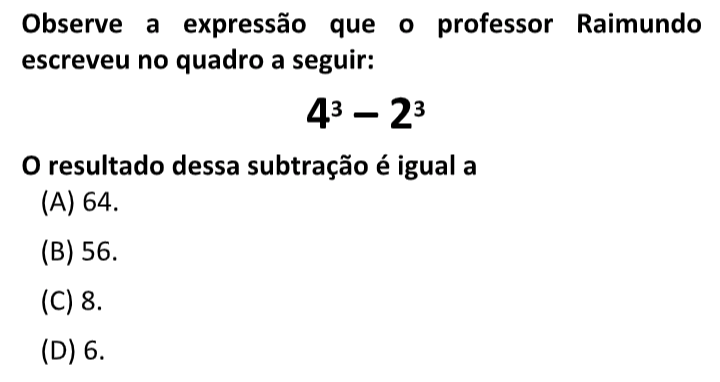
\includegraphics[scale=0.8]{qst18.59.png}
    \end{figure}
\end{frame}
% Question 2
\begin{frame}{Questão 2}
    \begin{figure}
        \caption{Área e volume}
        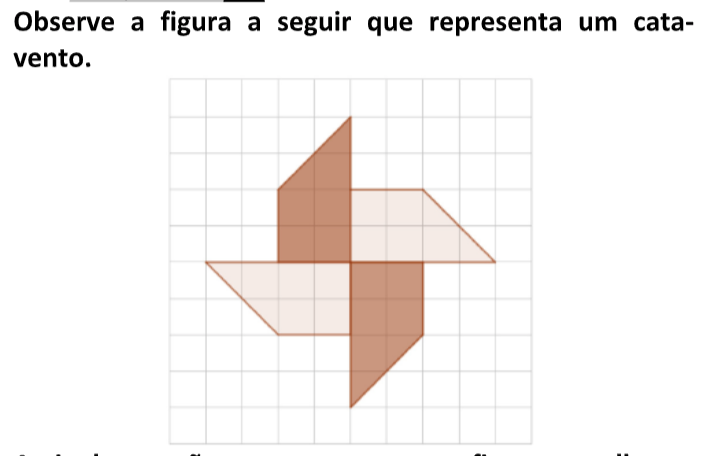
\includegraphics[scale=0.6]{qst19.24.png}
    \end{figure}
\end{frame}
% Question 3
\begin{frame}{Questão 3}
    \begin{figure}
        \caption{Área e volume}
        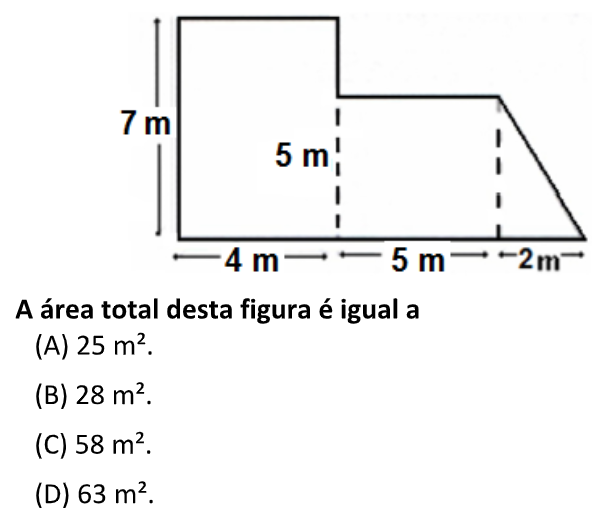
\includegraphics[scale=0.6]{qst19.51.png}
    \end{figure}
\end{frame}
% Question 4
\begin{frame}{Questão 4}
    \begin{figure}
        \caption{Razão e proporção}
        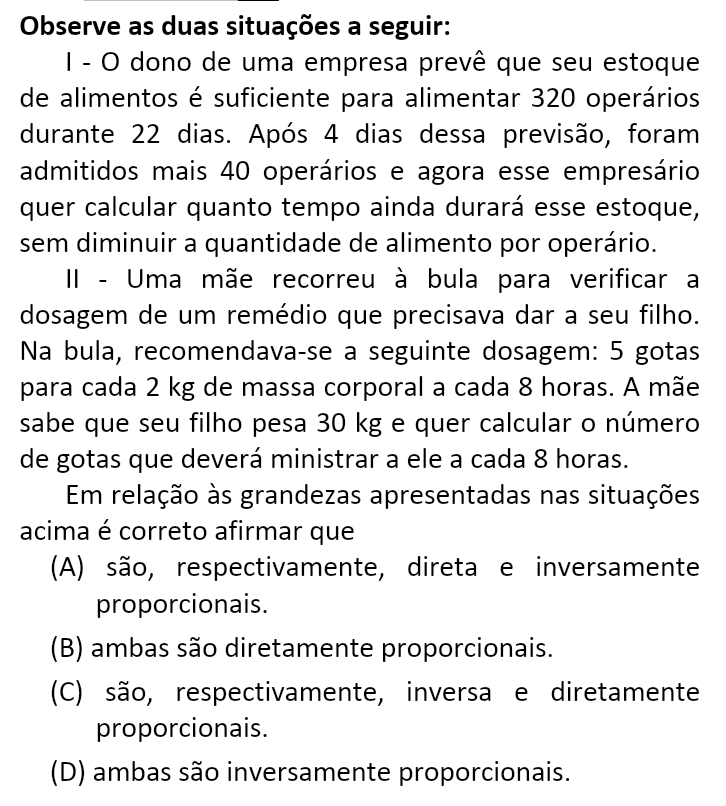
\includegraphics[scale=0.4]{qst20.14.png}
    \end{figure}
\end{frame}
% Question 5
\begin{frame}{Questão 5}
    \begin{figure}
        \caption{Geometria}
        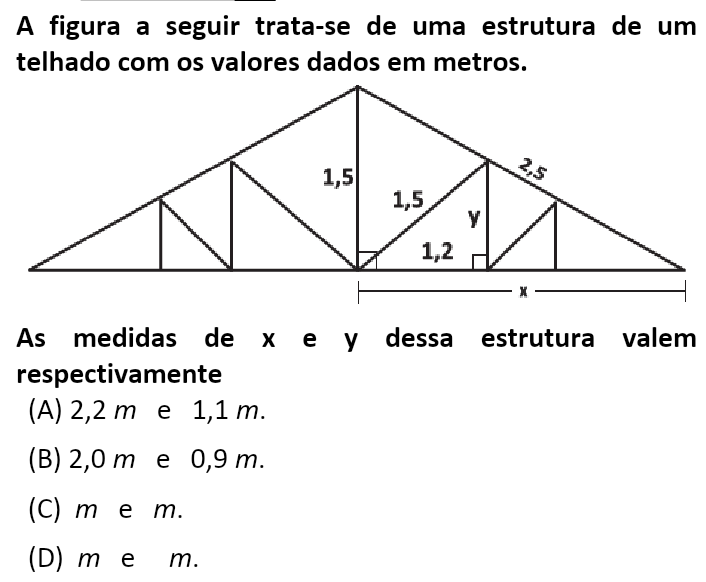
\includegraphics[scale=0.6]{qst20.37.png}
    \end{figure}
\end{frame}
% Question 6
\begin{frame}{Questão 6}
    \begin{figure}
        \caption{Geometria}
        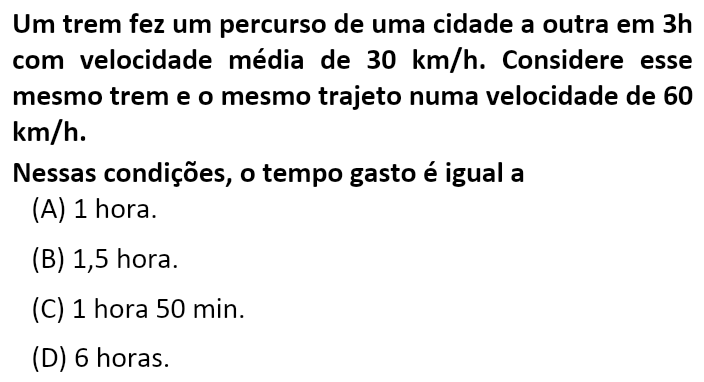
\includegraphics[scale=0.8]{qst20.55.png}
    \end{figure}
\end{frame}
% Question 7
\begin{frame}{Questão 7}
    \begin{figure}
        \caption{Geometria}
        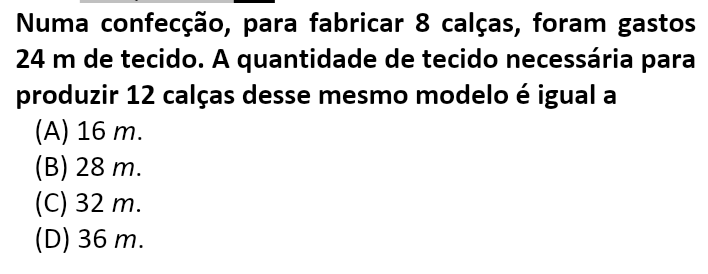
\includegraphics[scale=0.8]{qst21.23.png}
    \end{figure}
\end{frame}
% Question 8
\begin{frame}{Questão 8}
    \begin{figure}
        \caption{Geometria}
        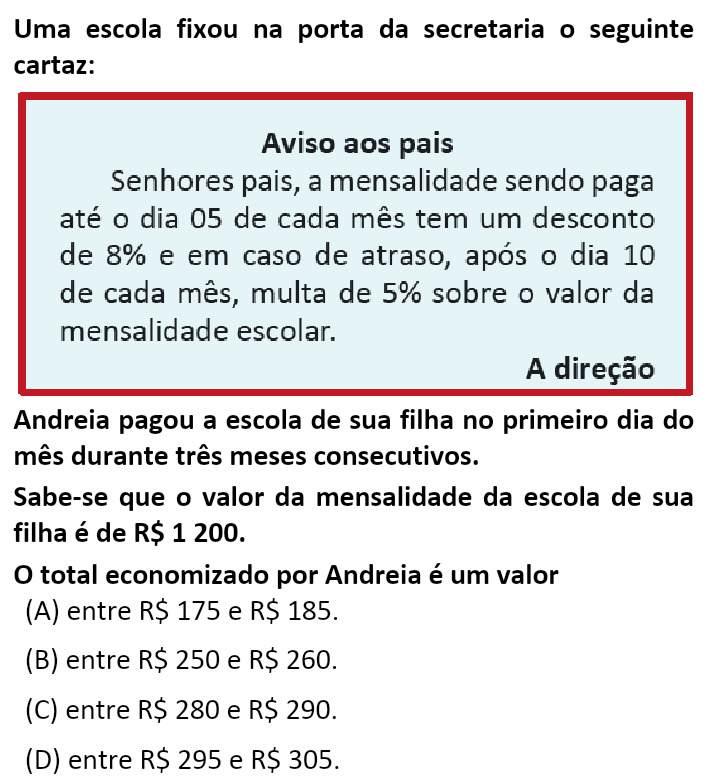
\includegraphics[scale=0.45]{qst22.01.png}
    \end{figure}
\end{frame}
% Question 9
\begin{frame}{Questão 9}
    \begin{figure}
        \caption{Lógica}
        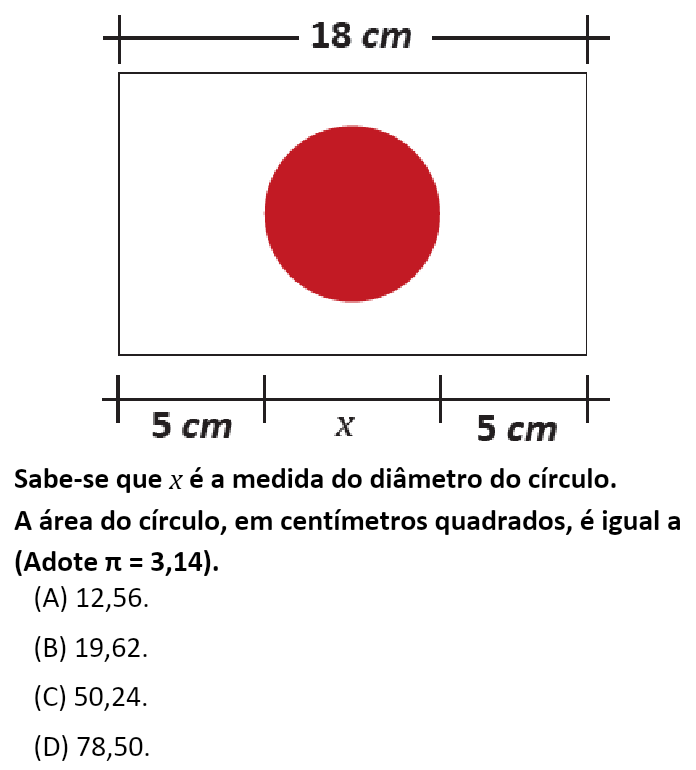
\includegraphics[scale=0.45]{qst22.31.png}
    \end{figure}
\end{frame}
% Question 10
\begin{frame}{Questão 10}
    \begin{figure}
        \caption{Geometria}
        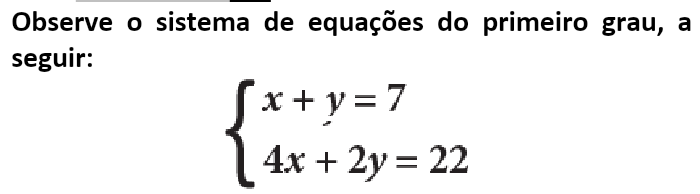
\includegraphics[scale=0.8]{qst22.53.png}
    \end{figure}
    \begin{center}
        Faça o gráfico das equações acima.
    \end{center}
\end{frame}
% Question 11
\begin{frame}{Questão 11}
    \begin{columns}[T] % align columns
        \begin{column}{.6\textwidth}
            \begin{figure}
                \caption{Lógica}
                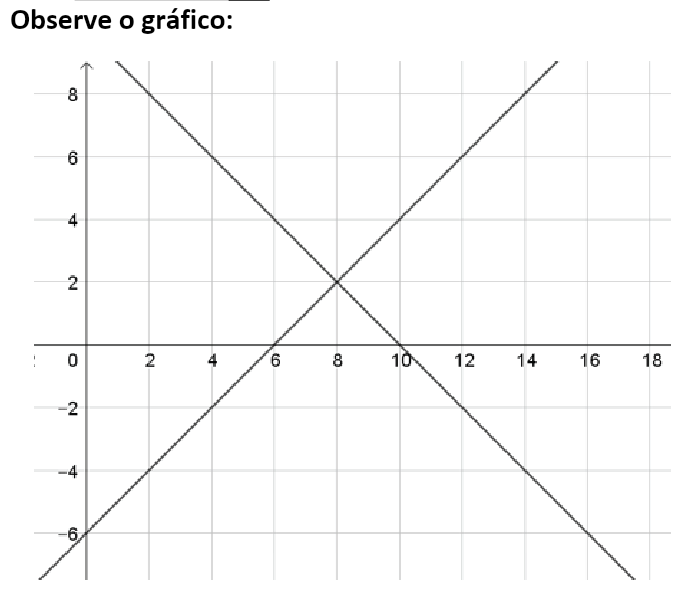
\includegraphics[scale=0.5]{qst23.10.png}
            \end{figure}
        \end{column}%
        %
        \hfill%
        %
        \begin{column}{.5\textwidth}
            \begin{figure}[h]
                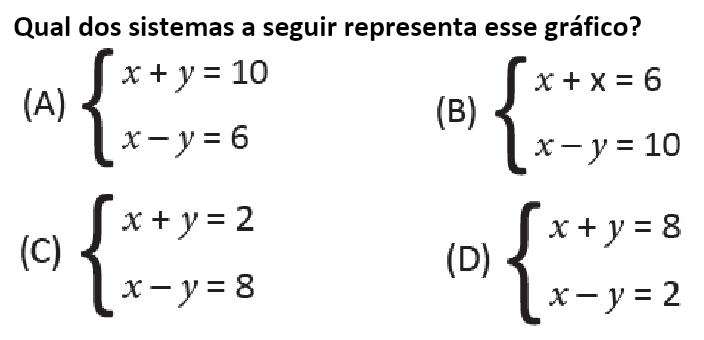
\includegraphics[scale=0.4]{qst23.17.png}
            \end{figure}
        \end{column}%
    \end{columns}
\end{frame}
% Question 12
\begin{frame}{Questão 12}
    \begin{figure}
        \caption{Lógica}
        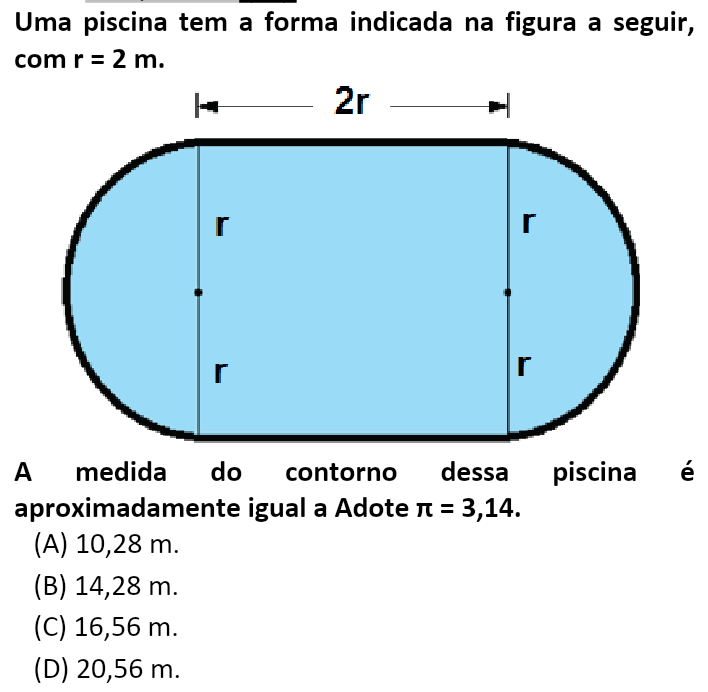
\includegraphics[scale=0.45]{qst23.38.png}
    \end{figure}
\end{frame}
% Question 13
\begin{frame}{Questão 13}
    \begin{figure}
        \caption{Lógica}
        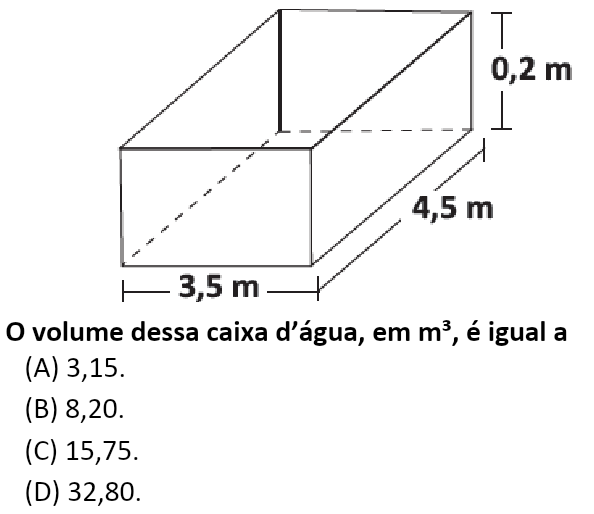
\includegraphics[scale=0.6]{qst23.54.png}
    \end{figure}
\end{frame}
% Question 14
\begin{frame}{Questão 14}
    \begin{figure}
        \caption{Lógica}
        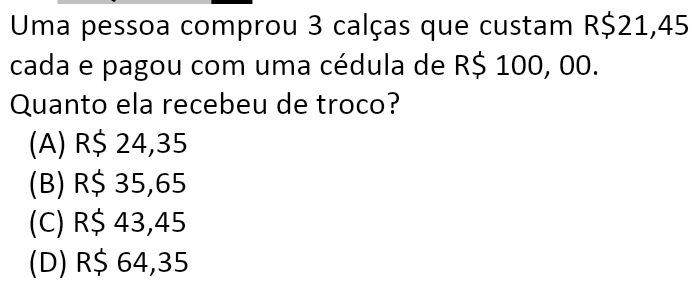
\includegraphics[scale=0.8]{qst24.16.png}
    \end{figure}
\end{frame}
% Question 15
\begin{frame}{Questão 15}
    \begin{figure}
        \caption{Lógica}
        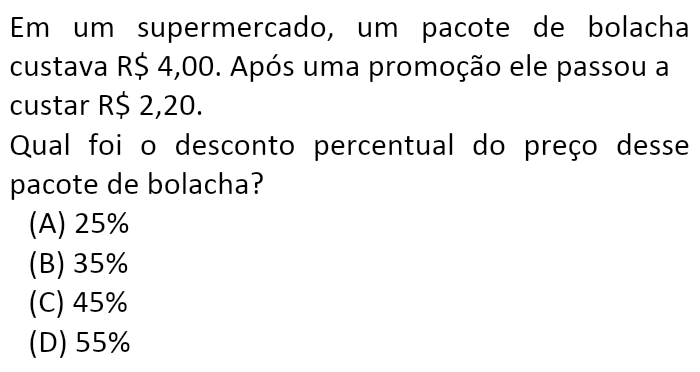
\includegraphics[scale=0.8]{qst24.38.png}
    \end{figure}
\end{frame}
% Question 16
\begin{frame}{Questão 16}
    \begin{figure}
        \caption{Lógica}
        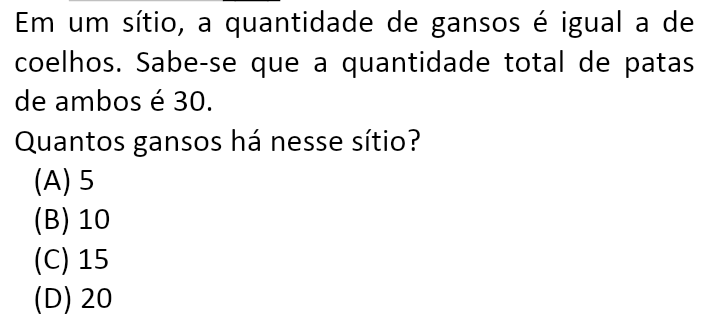
\includegraphics[scale=0.8]{qst25.41.png}
    \end{figure}
\end{frame}
% Question 17
\begin{frame}{Questão 17}
    \begin{figure}
        \caption{Lógica}
        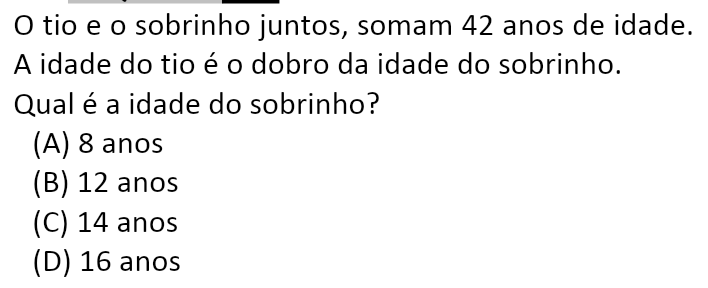
\includegraphics[scale=0.8]{qst25.56.png}
    \end{figure}
\end{frame}
%%%%%%%%%%%%%%%
\subsection{Grandezas}
%
\subsection{Análise dimensional}
%
\subsection{Notação científica}
%
\subsection{Múltiplos e submúltiplos}
%%
\section{Movimento}

\end{document}